%----------------------------------------------------------------------------------------
%
% A LaTeX-template for 1DV510. Modified and translated by Björn Lindenberg at LNU.
% Based on an original master thesis template created by Marcus Wilhelmsson at LNU.
%
%----------------------------------------------------------------------------------------

% Settings and document configuration

\documentclass[a4paper,12pt]{article} 
\usepackage[T1]{fontenc} 
\usepackage{times} 
\usepackage[swedish,english]{babel} 
\usepackage[utf8]{inputenc} 
\usepackage{dtk-logos} 
\usepackage{wallpaper} 
\usepackage[absolute]{textpos} 
\usepackage[top=2cm, bottom=2.5cm, left=3cm, right=3cm]{geometry} 
\usepackage[parfill]{parskip} 
\usepackage{csquotes} 
\usepackage{float} 
\usepackage{lipsum} % Used for dummy text. Can be removed.
\usepackage{listings, color}
\usepackage{graphicx}

\lstdefinestyle{Asm}{
  belowcaptionskip=1\baselineskip,
  breaklines=true,
  frame=L,
  xleftmargin=\parindent,
  language=[x86masm]Assembler,
  showstringspaces=false,
  basicstyle=\footnotesize\ttfamily,
  keywordstyle=\bfseries\color{purple!40!black},
  commentstyle=\itshape\color{green!40!black},
  identifierstyle=\color{blue},
  stringstyle=\color{orange},
}

% Fontsizes for section headings.
\usepackage{sectsty} 
\sectionfont{\fontsize{14}{15}\selectfont}
\subsectionfont{\fontsize{12}{15}\selectfont}
\subsubsectionfont{\fontsize{12}{15}\selectfont}

%----------------------------------------------------------------------------------------
%	This part is used for the text box on the title page
%----------------------------------------------------------------------------------------
\newsavebox{\mybox}
\newlength{\mydepth}
\newlength{\myheight}

\newenvironment{sidebar}%
{\begin{lrbox}{\mybox}\begin{minipage}{\textwidth}}%
{\end{minipage}\end{lrbox}%
 \settodepth{\mydepth}{\usebox{\mybox}}%
 \settoheight{\myheight}{\usebox{\mybox}}%
 \addtolength{\myheight}{\mydepth}%
 \noindent\makebox[0pt]{\hspace{-20pt}\rule[-\mydepth]{1pt}{\myheight}}%
 \usebox{\mybox}}

%----------------------------------------------------------------------------------------
%	Title
%----------------------------------------------------------------------------------------
\newcommand\BackgroundPic{
    \put(-2,-3){
    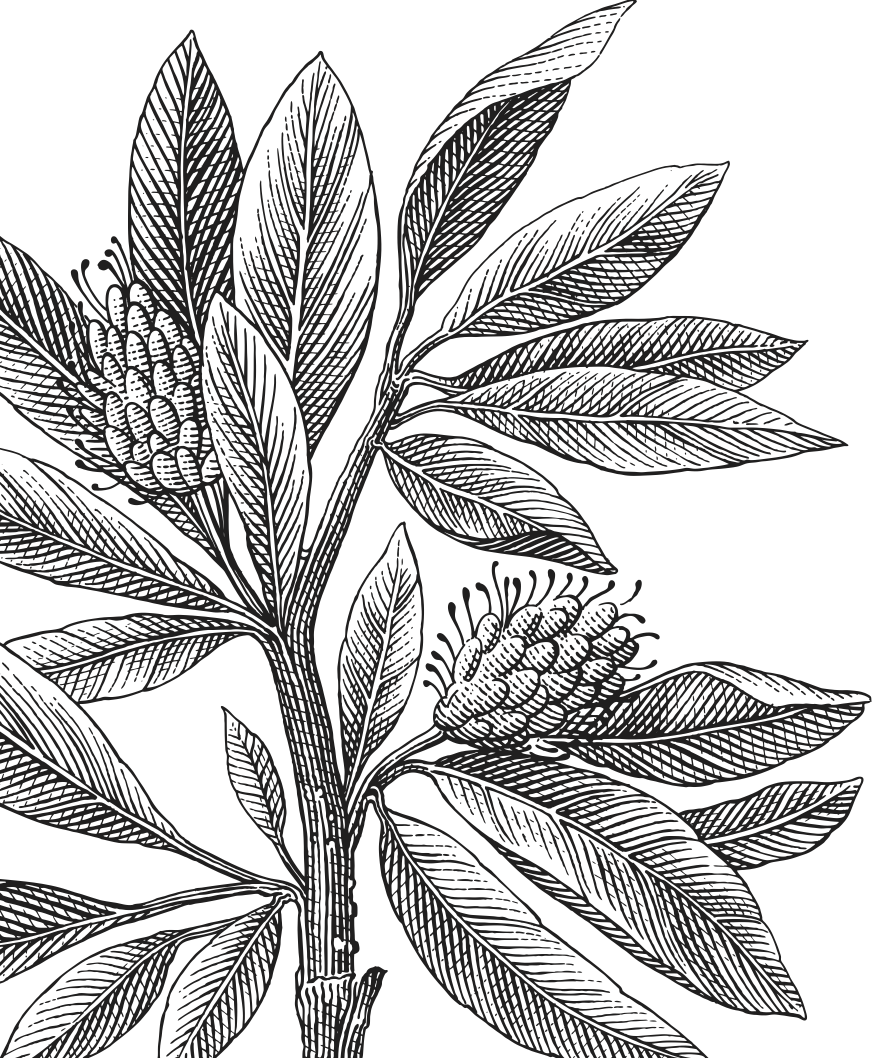
\includegraphics[keepaspectratio,scale=0.3]{img/lnu_etch.png} % Background image
    }
}
\newcommand\BackgroundPicLogo{
    \put(30,740){
    
\includegraphics[keepaspectratio,scale=0.10]{img/logo.png} % LNU logo
    }
}

\title{
\vspace{-8cm}
\begin{sidebar}
    \vspace{10cm}
    \normalfont \normalsize
    \huge Computer Technology I\\ % Main title
    \vspace{-1.3cm}
\end{sidebar}
\vspace{3cm}
\begin{flushleft}
    \huge Lab. 1 : How to use the PORTs, Digital input/output, Subroutine call % Subtitle
     \small \\ \emph{}
\end{flushleft}
\null
\vfill
\begin{textblock}{5}(10,13)
\begin{flushright}
\begin{minipage}{\textwidth}
\begin{flushleft} \large
\emph{Authors:}\textsc{ Leonardo PEDRO, Loïc GALLAND}\\  % Author
\emph{Supervisor:}  \textsc{} \\  % Author
\emph{Semester:} Autumn 2019\\ % Semester
\emph{Area:} Computer Science \\ % Area
\emph{Course code:} 1DT301 % Course
\end{flushleft}
\end{minipage}
\end{flushright}
\end{textblock}
}

\date{} % Empty date command. Use \today inside for today's date.
\author{} % Normally one would use this to define authors. However in this case the title command takes care of everything, so we leave the field empty to get rid of warnings. 

\begin{document}

\pagenumbering{gobble} % Turn off page numbering
\newgeometry{left=5cm}
\AddToShipoutPicture*{\BackgroundPic} % Adds the background image to the title page
\AddToShipoutPicture*{\BackgroundPicLogo} % Adds the logo to the title page
\maketitle % Prints the title
\restoregeometry
\clearpage

\pagenumbering{roman} % Roman page numbering for abstract page


\selectlanguage{english}

\newpage

\pagenumbering{gobble} % Turn off page numbering
\tableofcontents 

\newpage
\pagenumbering{arabic} % Turn on page numbering


\section{Task 1}

\textit{Write a program in Assembly language to light LED 2.
You can use any of the four ports, but start with PORTB.
The program should be very short! How many instructions is minimum number?}

\lstset{style=Asm}
\begin{lstlisting}
;>>>>>>>>>>>>>>>>>>>>>>>>>>>>>>>>>>>>>>>>>>>>>>>>>>>>>>>>>>>
; 1DT301, Computer Technology I
; Date: 2019-09-09
; Author:
; Loic GALLAND
; Leonardo PEDRO
;
; Lab number: 1
; Title: How to use the PORTs. Digital input/output. Subroutine call.
;
; Hardware: STK600, CPU ATmega2560
;
; Function: Program to light up the LED number 2

; Input ports: NO inputs ports in this Task
;
; Output ports: The portB is used as an output port
;
; Subroutines: If applicable.
; Included files: m2560def.inc
;
; Other information:
;
; Changes in program: (Description and date)
;
;<<<<<<<<<<<<<<<<<<<<<<<<<<<<<<<<<<<<<<<<<<<<<<<<<<<<<<<<<<<

.includes "m2560def.inc"
ldi r16, 0xFF
out DDRB, r16

ldi r16 , 0b11111011
out portB, r16
\end{lstlisting}
To be able to light up the LEDs we need 4 lines of code. The first line is to store into the register r16 the value 0xFF. In the second line the register r16 is loaded to DDRB (Data Direction Register of port B). In the third line the desired binary code is stored into register r16. The binary number will determine which LED will light up. In the last line the register r16 is loaded into the PortB (Data Register of Port B).
\newpage
This is the flowchart of the task 1:
\begin{center}
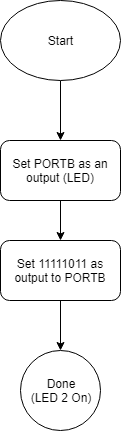
\includegraphics{img/Task1.png}
\end{center}

\newpage
\section{Task 2}
Write a program in Assembly language to read the switches and light the corresponding
LED.
Example: When you press SW5, LED5 so should light.
Make an initialization part of the program and after that an infinite loop.
\lstset{style=Asm}
\begin{lstlisting}
;>>>>>>>>>>>>>>>>>>>>>>>>>>>>>>>>>>>>>>>>>>>>>>>>>>>>>>>>>>>
; 1DT301, Computer Technology I
; Date: 2019-09-09
; Author:
; Loic GALLAND
; Leonardo PEDRO
;
; Lab number: 1
; Title: How to use the PORTs. Digital input/output. Subroutine call.
;
; Hardware: STK600, CPU ATmega2560
;
; Function: Program to light up the LED correponding to the switch. EX: (Switch number 1 will light up LED number 1)

; Input ports: PortA is used as input to get the information from the switches 
;
; Output ports: The portB is used as an output ports to control the LEDs
;
; Subroutines: If applicable.
; Included files: m2560def.inc
;
; Other information:
;
; Changes in program: (Description and date)
;
;<<<<<<<<<<<<<<<<<<<<<<<<<<<<<<<<<<<<<<<<<<<<<<<<<<<<<<<<<<<

.include "m2560def.inc"
ldi r16, 0xFF 		;Setting up the data direction for Port B
out DDRB, r16 		;Set port B as output

ldi r16, 0x00 		;Setting up the data direction for Port A
out DDRA, r16 		;Set Port A as output

my_loop:		;Loop to always check which switch is pressed
	in r17,PINA ;Getting the information of which switch is pressed
	out portB, R17 	;Lighting up the corresponding LED
rjmp my_loop
\end{lstlisting}
\newpage
This is the flowchart for Task 2:
\begin{center}
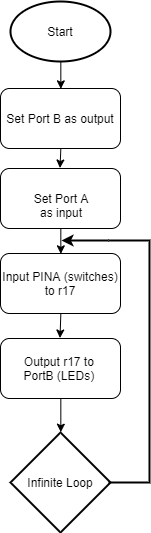
\includegraphics{img/Task2.png}
\end{center}
\newpage
\section{Task 3}
This is the code for the third task:
\lstset{style=Asm}
\begin{lstlisting}
;>>>>>>>>>>>>>>>>>>>>>>>>>>>>>>>>>>>>>>>>>>>>>>>>>>>>>>>>>>>
; 1DT301, Computer Technology I
; Date: 2019-09-09
; Author:
; Loic GALLAND
; Leonardo PEDRO
;
; Lab number: 1
; Title: How to use the PORTs. Digital input/output. Subroutine call.
;
; Hardware: STK600, CPU ATmega2560
;
; Function: Program to only light up LED number 0 if the switch number 5 is pressed. If any other switch is pressed, nothing will happen

; Input ports: The Port A will be used as an input port in this Task
;
; Output ports: The portB is used as an output port
;
; Subroutines: If applicable.
; Included files: m2560def.inc
;
; Other information:
;
; Changes in program: (Description and date)
;
ldi r16, 0xFF 		;Setting up the data direction for Port B
out DDRB, r16 		;Set port B as output

ldi r16, 0x00 		;Setting up the data direction for Port A
out DDRA, r16 		;Set Port A as output

ldi r16, 0xFF		;Turn off all the LEDs
out portB, r16

ldi r18, 0b11011111
ldi r19, 0b11111110

my_loop:
	in r17, PINA 	;get the info from the switch
	cp r17, r18 	;compare switch info with desired one 
	breq light 	;condition if r17=r18 go to the "light"
rjmp my_loop

light: out portB,r19	;turns on the LED0
\end{lstlisting}

\newpage
\section{Task 5}
This is the code for the fifth task:
\lstset{style=Asm}
\begin{lstlisting}
;>>>>>>>>>>>>>>>>>>>>>>>>>>>>>>>>>>>>>>>>>>>>>>>>>>>>>>>>>>>
; 1DT301, Computer Technology I
; Date: 2019-09-09
; Author:
; Loic GALLAND
; Leonardo PEDRO
;
; Lab number: 1
; Title: How to use the PORTs. Digital input/output. Subroutine call.
;
; Hardware: STK600, CPU ATmega2560
;
; Function: Create a program that creates a Ring Counter with a delay of approximately 0.5 seconds between each step. 

; Input ports: NO inputs ports in this Task
;
; Output ports: The portB is used as an output port
;
; Subroutines: A subroutine will be used when creating the 0.5 second delay. 
; Included files: m2560def.inc
;
;<<<<<<<<<<<<<<<<<<<<<<<<<<<<<<<<<<<<<<<<<<<<<<<<<<<<<<<<<<<

.includes "m2560def.inc"

; Initialize SP, Stack Pointer
ldi r20, HIGH(RAMEND)	; R20 = high part of RAMEND address
out SPH,R20 		; SPH = high part of RAMEND address
ldi R20, low(RAMEND) 	; R20 = low part of RAMEND address
out SPL,R20 		; SPL = low part of RAMEND address

ldi r16, 0xFF 		;Setting up the data direction for Port B
out DDRB, r16 		;Set port B as output

ldi r17, 0b11111110 	;Initial LED state
out PortB, r17

my_loop:
	out portB, r17
	CALL Delay
	com r17
	LSL r17
	com r17
rjmp my_loop

Delay:
;Generated by delay loop calculator
:at http://www.bretmulvey.com/avrdelay.html
;
;Delay 4 050 000 cycles
;500ms at 8.1 MHz

	ldi r18, 21
	ldi r19, 140
	ldi 20, 174
L1:	dec r20
	brne L1
	dec r19
	brne L1
	dec r18
	brne L1
	rjmp PC+1
RET
\end{lstlisting}

\newpage
\section{Task 6}
This is the code for the sixth task:
\lstset{style=Asm}
\begin{lstlisting}
;>>>>>>>>>>>>>>>>>>>>>>>>>>>>>>>>>>>>>>>>>>>>>>>>>>>>>>>>>>>
; 1DT301, Computer Technology I
; Date: 2019-09-09
; Author:
; Loic GALLAND
; Leonardo PEDRO
;
; Lab number: 1
; Title: How to use the PORTs. Digital input/output. Subroutine call.
;
; Hardware: STK600, CPU ATmega2560
;
; Function: Creates a program that creates a Johnson Counter in an infinite loop

; Input ports: NO inputs ports in this Task
;
; Output ports: The portB is used as an output port
;
; Subroutines: To be able to use the delay
; Included files: m2560def.inc
;<<<<<<<<<<<<<<<<<<<<<<<<<<<<<<<<<<<<<<<<<<<<<<<<<<<<<<<<<<<

.includes "m2560def.inc"

; Initialize SP, Stack Pointer
ldi r20, HIGH(RAMEND)	; R20 = high part of RAMEND address
out SPH,R20 		; SPH = high part of RAMEND address
ldi R20, low(RAMEND) 	; R20 = low part of RAMEND address
out SPL,R20 		; SPL = low part of RAMEND address

ldi r16, 0xFF	;Setting up the date direction register for Port B
out DDRB, r16	;Set port B as output

ldi r16, 0xFF
out portB, r16

ldi r21, 0b11111110	;Initial LED state
ldi r22, 0xFF	;When all the LEDs are turned off 
ldi r23, 0x00	;When all the LEDs are turned on

my_loop:
	out portB, r21
	LSL r21
	CALL Delay
	;Compare the current status of the LEDs to check if they are all turned on. 
	cp r21, r23	
	breq light
rjmp my_loop

light:
	out portB, r23
	CALL Delay
	ldi r21, 0b10000000
	out portB, r21
	Second_loop:
		out portB, r21
		ASR r21
		CALL Delay
		cp r21, r22		;Compare the current status to know if it needs to start going the other way
		breq my_loop
	rjmp Second_loop

Delay:
;Generated by delay loop calculator
:at http://www.bretmulvey.com/avrdelay.html
;
;Delay 4 050 000 cycles
;500ms at 8.1 MHz

	ldi r18, 21
	ldi r19, 140
	ldi 20, 174
L1:	dec r20
	brne L1
	dec r19
	brne L1
	dec r18
	brne L1
	rjmp PC+1
RET
\end{lstlisting}


% Prints your bibliography database xxx.bib
\bibliographystyle{IEEEtran}
\bibliography{ref.bib}

\end{document}
